\documentclass{article}
\usepackage{spconf,amsmath,amssymb,graphicx,booktabs,multirow}
\usepackage[hidelinks]{hyperref}
\title{Heat-Kernel Structural Features for Cooperative Policy Learning}
\name{Gurui Jin$^{\star}$ \qquad Ercan Engin Kuruoglu$^{\star}$
\thanks{This work was supported in part by the National Natural Science Foundation of China under Grants 62388102 and 62571297 and by ...... Lab under Grant ..... The code is available at \url{https://github.com/jgr2021/HKS-MADDPG}. Corresponding author: Ercan Engin Kuruoglu (kuruoglu@sz.tsinghua.edu.cn).}}
\address{$^{\star}$ Tsinghua Shenzhen International Graduate School, Tsinghua University}
\newcommand{\R}{\mathbb{R}}
\newcommand{\obs}{\mathbf{o}}
\newcommand{\hks}{\mathbf{h}}
\begin{document}
\maketitle
\begin{abstract}
Cooperative navigation requires decentralized agents to coordinate target allocation from geometric observations. We study a lightweight heat kernel signature (HKS) that converts an observation-derived agent--landmark bipartite graph into three diffusion-return features appended to each actor input, without changing communication, replay, or critic interfaces. We characterize the structural information represented by these returns and evaluate the representation with MADDPG on three-agent/three-landmark simple spread across five training seeds. Relative to raw observations, HKS reduces mean assignment distance by 19.6\% and increases coverage-radius AUC by 26.9\%, while collision frequency rises; mean return changes from $-26.058$ to $-24.952$. Paired confidence intervals across seeds include zero, so these results describe a promising but variable coverage--collision trade-off.
\end{abstract}
\begin{keywords}
Graph signal processing, heat kernel signature, multi-agent reinforcement learning, cooperative navigation
\end{keywords}

\section{Introduction}
Cooperative navigation requires multiple agents to distribute themselves across targets while avoiding collisions. The usefulness of a nearby target depends on the positions of teammates: several agents approaching the same target can leave others unattended. Centralized-training, decentralized-execution methods such as MADDPG~\cite{lowe} and MAPPO~\cite{mappo} use centralized value estimation to support decentralized policies. In our setting, each actor can reconstruct the agent--landmark geometry from its relative-coordinate observation. This makes the policy input a natural place to encode shared-target relationships.

Observation design has been studied in swarm reinforcement learning, where mean embeddings organize information from multiple neighbors~\cite{swarm}. Relational reinforcement learning uses object-level reasoning for action selection~\cite{zambaldi}, while graph-based policies learn interaction features through aggregation~\cite{graphpg,gcrl}. Agent--entity message passing includes environmental objects in the relational model~\cite{emp}; InforMARL aggregates local graph information for both actors and critics~\cite{informarl}. Heat diffusion has also been used to propagate messages over a learned agent graph~\cite{cdc}. Together, these studies motivate a representation that summarizes how agents and targets are related at the current step.

Graph diffusion provides such a summary through spectral functions of the graph Laplacian~\cite{shuman}. The heat kernel signature (HKS) describes diffusion at a focal node across scales~\cite{sun}, and GraphWave uses diffusion wavelets to represent structural roles~\cite{graphwave}. Random-walk returns provide related node encodings in LSPE~\cite{lspe}; GraphGPS treats structural encodings as a design component alongside message passing and attention~\cite{graphgps}. In an agent--landmark bipartite graph, diffusion returns have a direct task interpretation: alternating paths connect the focal agent to teammates through shared landmarks.

We construct a weighted agent--landmark graph from each actor's observation and append three focal HKS values to the original policy input. The resulting feature is a deterministic summary of current geometry within the existing decentralized observation and CTDE interfaces. We derive how weighted return paths encode relations through shared landmarks and characterize the descriptor's transformation properties. A five-seed comparison with raw-observation MADDPG then measures coverage, assignment distance, collisions, and return. HKS yields better mean coverage and assignment distance alongside more frequent collisions, with variability across seeds.

\section{Problem Formulation}
\begin{figure}[t]
\centering
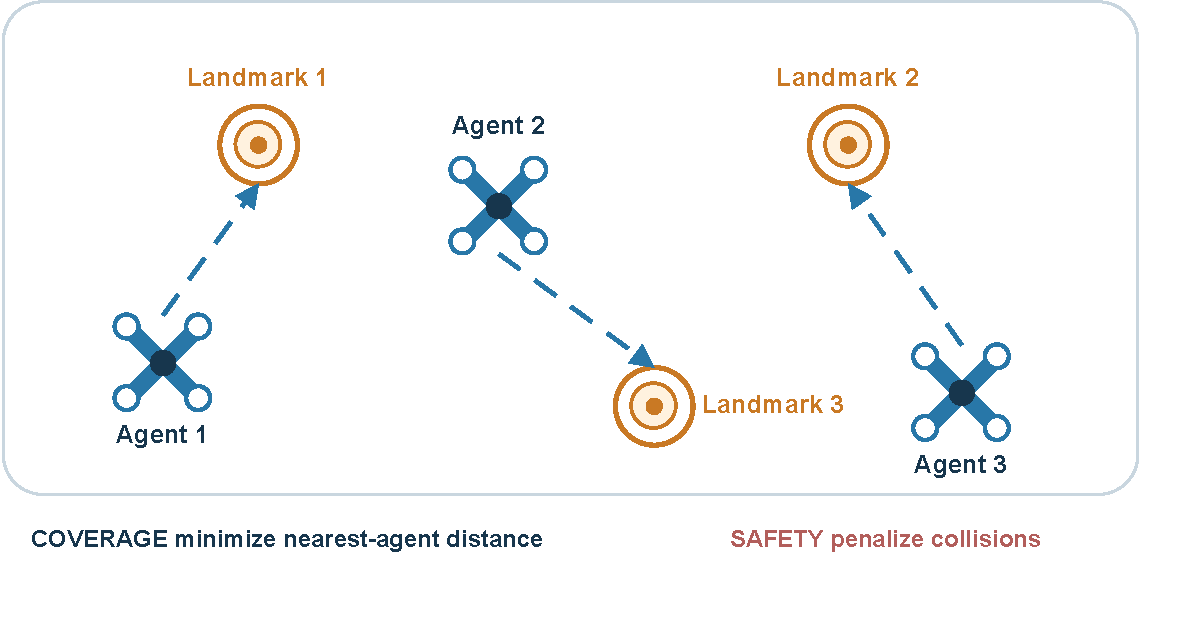
\includegraphics[width=\columnwidth]{figure1_task.pdf}
\caption{Three-agent cooperative-navigation task with three landmarks. Dashed arrows illustrate possible target assignments; the team seeks landmark coverage while avoiding agent--agent collisions.}
\label{fig:task}
\end{figure}
As illustrated in Fig.~\ref{fig:task}, we consider the standard cooperative-navigation simple spread task~\cite{lowe} with $N=3$ movable agents and $M=3$ fixed landmarks in a two-dimensional workspace. Let $p_i^t,v_i^t\in\R^2$ denote the position and velocity of agent $i$ at step $t$, and let $\ell_m\in\R^2$ denote landmark $m$. Each episode lasts $T=25$ steps. An agent chooses one of five discrete movement actions (no-op and motion along the two coordinate axes). The task objective is to bring the team close to all landmarks while avoiding agent--agent collisions.

The standard environment reward reflects these two requirements. The shared coverage term is determined by the distance from each landmark to its nearest agent,
\begin{equation}
 r_{\mathrm{cov}}^t=-\sum_{m=1}^{M}\min_{j\in\{1,\ldots,N\}}\|p_j^t-\ell_m\|_2,
\end{equation}
while colliding agents receive an additional penalty. Writing $I_{ij}^t$ for the collision indicator, an agent reward can be expressed as
\begin{equation}
 r_i^t=r_{\mathrm{cov}}^t-\lambda_{\mathrm{col}}\sum_{j\neq i}I_{ij}^t,
\end{equation}
with the environment's fixed collision weight $\lambda_{\mathrm{col}}$. Successful behavior therefore requires joint optimization of landmark coverage and inter-agent spatial separation.

Each agent receives an 18-D observation
\begin{equation}
 o_i^t=\big[v_i^t,p_i^t,\{\ell_m-p_i^t\}_{m=1}^{3},\{p_j^t-p_i^t\}_{j\neq i},\{c_j^t\}_{j\neq i}\big],
\end{equation}
where $c_j^t$ denotes the environment-provided communication entry. The relative coordinates contain enough information to reconstruct the instantaneous agent--landmark geometry. Under centralized training with decentralized execution, actor $\pi_i$ selects $a_i^t$ from $o_i^t$, while critic $Q_i$ may use the joint observations and actions during training as in MADDPG~\cite{lowe}. The learning objective is
\begin{equation}
 J=\mathbb{E}\left[\sum_{t=0}^{T-1}\gamma^t\frac{1}{N}\sum_{i=1}^{N}r_i^t\right].
\end{equation}
Given the decentralized observation $o_i^t$, we seek a compact representation $z_i^t=f(o_i^t)$ that summarizes the instantaneous relations among the focal agent, its teammates, and the landmarks, and can be used together with $o_i^t$ for decentralized action selection.

\section{Proposed Method}
\begin{figure*}[t]
\centering
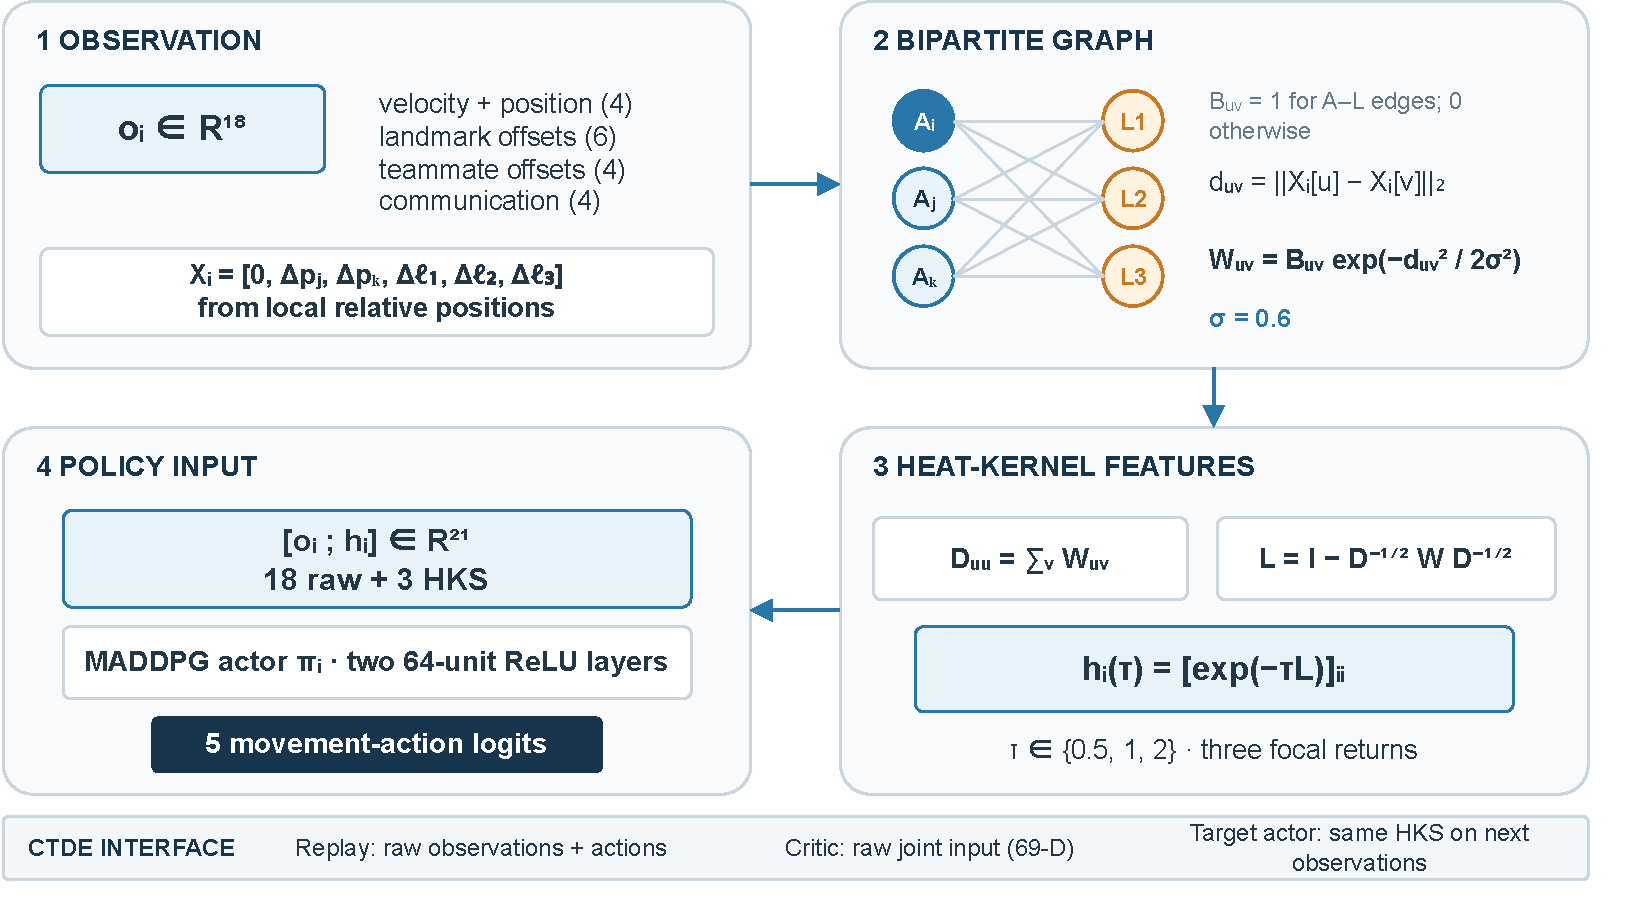
\includegraphics[width=\textwidth]{figure2_hks_actor.pdf}
\caption{Actor-side HKS augmentation. The local observation defines a weighted agent--landmark bipartite graph with Gaussian bandwidth $\sigma=0.6$. The normalized-Laplacian heat kernel gives three focal values at diffusion times $\tau\in\{0.5,1,2\}$, which are appended to the 18-D actor input. Replay and the centralized critic use raw observations and actions.}
\label{fig:method_overview}
\end{figure*}
\subsection{Observation-Derived Agent--Landmark Graph}
For focal agent $i$, all node positions are written in its local coordinate frame,
\begin{equation}
 X_i=[\mathbf{0},p_j-p_i,p_k-p_i,\ell_1-p_i,\ell_2-p_i,\ell_3-p_i]^\top,
\end{equation}
where $j,k\neq i$. Only fields already contained in the observation are used. Agents and landmarks form the two partitions of a complete bipartite graph. Its symmetric mask has $B_{uv}=1$ for agent--landmark pairs and $B_{uv}=0$ for all other pairs, including self-pairs. The weighted adjacency is
\begin{equation}
 W_{i,uv}=B_{uv}\exp\left(-\frac{\|X_{i,u}-X_{i,v}\|_2^2}{2\sigma^2}\right),\qquad \sigma=0.6.
\end{equation}
Thus the graph topology is fixed while the weights adapt deterministically to the current geometry.

\subsection{Heat-Kernel Structural Descriptor}
Let $D_i$ be the weighted-degree matrix, with $(D_i)_{uu}=\sum_v W_{i,uv}$, and
\begin{equation}
 L_i=I-D_i^{-1/2}W_iD_i^{-1/2}=U_i\Lambda_iU_i^\top.
\end{equation}
For the focal node, indexed by 0, the heat-kernel diagonal is
\begin{equation}
 h_i(\tau)=[e^{-\tau L_i}]_{00}=\sum_{q=1}^{6}e^{-\tau\lambda_{i,q}}U_{i,0q}^{2}.
\end{equation}
We use three diffusion times and define
\begin{equation}
 \mathbf{h}_i=[h_i(0.5),h_i(1),h_i(2)]^\top.
\end{equation}
The actor input therefore changes from 18 to 21 dimensions. The feature extractor has no trainable graph parameters; the raw observation is retained to preserve directional, velocity, and other information not recoverable from three scalar returns.

\subsection{Diffusion-Return Interpretation}
Writing $S=D^{-1/2}WD^{-1/2}$ gives $L=I-S$. Because the graph is bipartite, odd-length diagonal walks vanish and
\begin{equation}
 h_i(\tau)=e^{-\tau}\sum_{k=0}^{\infty}\frac{\tau^{2k}}{(2k)!}(S^{2k})_{00}.
\end{equation}
The first geometry-dependent term is
\begin{equation}
 (S^2)_{00}=\sum_m\frac{W_{0m}^{2}}{D_{00}D_{mm}}.
\end{equation}
Here $D_{mm}$ depends on the affinities between landmark $m$ and all agents. Hence even the lowest nonconstant return term combines the focal agent--landmark relation with how strongly the same landmark is connected to teammates; higher terms aggregate longer alternating agent--landmark paths. The descriptor is invariant to common translation, orthogonal transformations, and role-preserving relabeling of nonfocal nodes because these operations preserve pairwise distances or conjugate the Laplacian. These invariances characterize the descriptor itself. The complete policy combines the descriptor with the raw observation, so its overall transformation behavior is determined by the full input representation.



\subsection{Integration with CTDE}
Each MADDPG actor uses $[o_i;\mathbf{h}_i]\in\R^{21}$ and outputs five action logits. The centralized critic retains
\begin{equation}
 Q_i(o_1,o_2,o_3,a_1,a_2,a_3),
\end{equation}
with dimension $3\times18+3\times5=69$. Target actors compute the same descriptor from next observations. Relative to the raw actor, the added inputs increase the actor parameter count by 198 parameters; this capacity change is included in the evaluated augmentation.



\clearpage
\section{Experiments}
\begin{table}[t]
\centering
\caption{Best-return checkpoint selected separately for each method and seed on a 100-episode bank, then evaluated on the common 500-episode bank. Mean $\pm$ sample standard deviation across five training seeds.}
\label{tab:results}
\small\setlength{\tabcolsep}{4pt}
\begin{tabular}{lcc}
\toprule
Metric & Raw MADDPG & HKS \\
\midrule
Return $\uparrow$ & $-26.058 \pm 2.207$ & $-24.952 \pm 1.912$ \\
Assignment distance $\downarrow$ & $0.292 \pm 0.076$ & $0.235 \pm 0.079$ \\
Coverage AUC $\uparrow$ & $0.384 \pm 0.111$ & $0.487 \pm 0.152$ \\
Collision (\%) $\downarrow$ & $6.04 \pm 1.39$ & $8.69 \pm 2.32$ \\
Full coverage (\%) $\uparrow$ & $0.52 \pm 0.56$ & $2.04 \pm 3.36$ \\
\bottomrule
\end{tabular}
\end{table}
\subsection{Experimental Setup}
Raw MADDPG and HKS-augmented MADDPG use the matched settings in Table~\ref{tab:setup}. For each training seed, checkpoints are evaluated every 20,000 steps on a common 100-episode selection bank; the checkpoint with the highest mean return is then evaluated without exploration on a disjoint 500-episode bank.

\begin{table}[t]
\centering
\caption{Task and training settings shared by both methods.}
\label{tab:setup}
\footnotesize\setlength{\tabcolsep}{4pt}
\begin{tabular}{ll}
\toprule
Parameter & Setting \\
\midrule
Task & Simple spread; 3 agents, 3 landmarks \\
Episode / actions & 25 steps / 5 discrete actions \\
Training seeds & 41--45 \\
Transitions per seed & $2\times10^6$ \\
Rollout environments / replay & 4 / $10^6$ transitions \\
Batch size / discount & 1024 / 0.95 \\
Actor and critic networks & Two 64-unit ReLU hidden layers \\
Actor / critic learning rate & 0.01 / 0.01 \\
Target-update coefficient & 0.01 \\
\bottomrule
\end{tabular}
\end{table}

Return is retained as an overall reward measure, while task-level metrics directly measure navigation behavior. Assignment distance is the minimum endpoint average distance under a one-to-one agent--landmark matching. Target coverage rate is the fraction of landmarks covered at the episode endpoint using the environment's evaluation threshold. Figure~\ref{fig:coverage_training} tracks this quantity throughout training. We additionally report coverage-radius AUC, which averages coverage over radii from 0.05 to 0.30, and collision-step rate, the fraction of steps with at least one agent collision.

\begin{figure}[t]
\centering
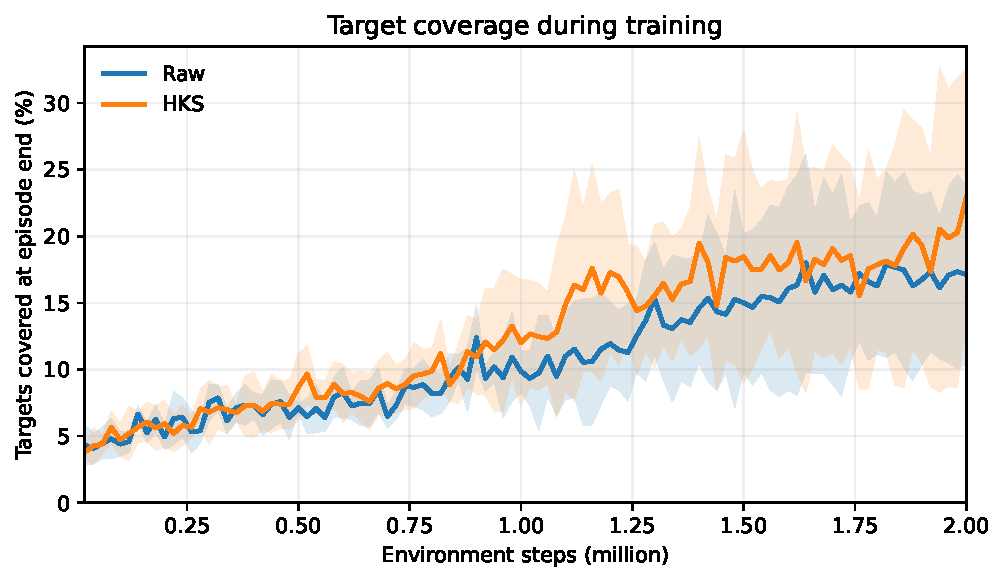
\includegraphics[width=\columnwidth]{target_coverage_over_training.pdf}
\caption{Target coverage during training. At each evaluation checkpoint, coverage is the fraction of landmarks covered at the episode endpoint, averaged across five training seeds; shaded bands show 95\% intervals across seeds.}
\label{fig:coverage_training}
\end{figure}

\subsection{Results and uncertainty}
Figure~\ref{fig:coverage_training} tracks endpoint target coverage during training; HKS has higher mean coverage through much of the later stage. At the selected checkpoints, Table~\ref{tab:results} shows a decrease in mean one-to-one assignment distance from 0.292 to 0.235 (19.6\%) and an increase in coverage-radius AUC from 0.384 to 0.487 (26.9\%). Mean return changes from $-26.058$ to $-24.952$. HKS improves return, assignment distance, and coverage AUC in three of the five paired seeds, rather than uniformly.

The mean collision-step rate rises from 6.04\% to 8.69\%; it is higher for HKS in four of five seeds. Full three-landmark endpoint coverage remains rare (0.52\% versus 2.04\%). The paired HKS-minus-raw return difference is $1.106$, with a two-sided Student-$t$ 95\% confidence interval of $[-2.021,4.234]$ across the five seeds. The corresponding intervals for assignment distance, coverage AUC, and collision frequency also include zero. Thus the observed geometric gains and collision cost are descriptive trends, not established population-level improvements.

As a separate checkpoint-selection sensitivity check, the original 500-episode final-step evaluations give mean returns of $-25.732$ (Raw) and $-25.664$ (HKS), a much smaller difference than the selected-checkpoint result. These final-step evaluations used a separate scene bank and are not pooled with Table~\ref{tab:results}. The reported evidence is specific to these two MADDPG representations, this task, and the stated selection protocol.

\section{Conclusion}
We introduced an actor-side HKS representation that converts observation-derived agent--landmark geometry into three diffusion-return features while preserving the original CTDE information interfaces. The return expansion explains how shared landmarks couple focal and teammate geometry. In five-seed MADDPG experiments, HKS has lower mean assignment distance and higher mean coverage, alongside increased collision exposure; paired uncertainty remains substantial. This comparison characterizes the resulting coverage--collision trade-off under the stated task and selection protocol.

\clearpage
\bibliographystyle{IEEEbib}
\bibliography{references}
\end{document}
